\subsection*{Дополнительное пояснение к смещению и разбросу}

Довольно популярной интерпретацией смещения и разброса является следующее изображение:
\begin{figure}[H]
    \centering
    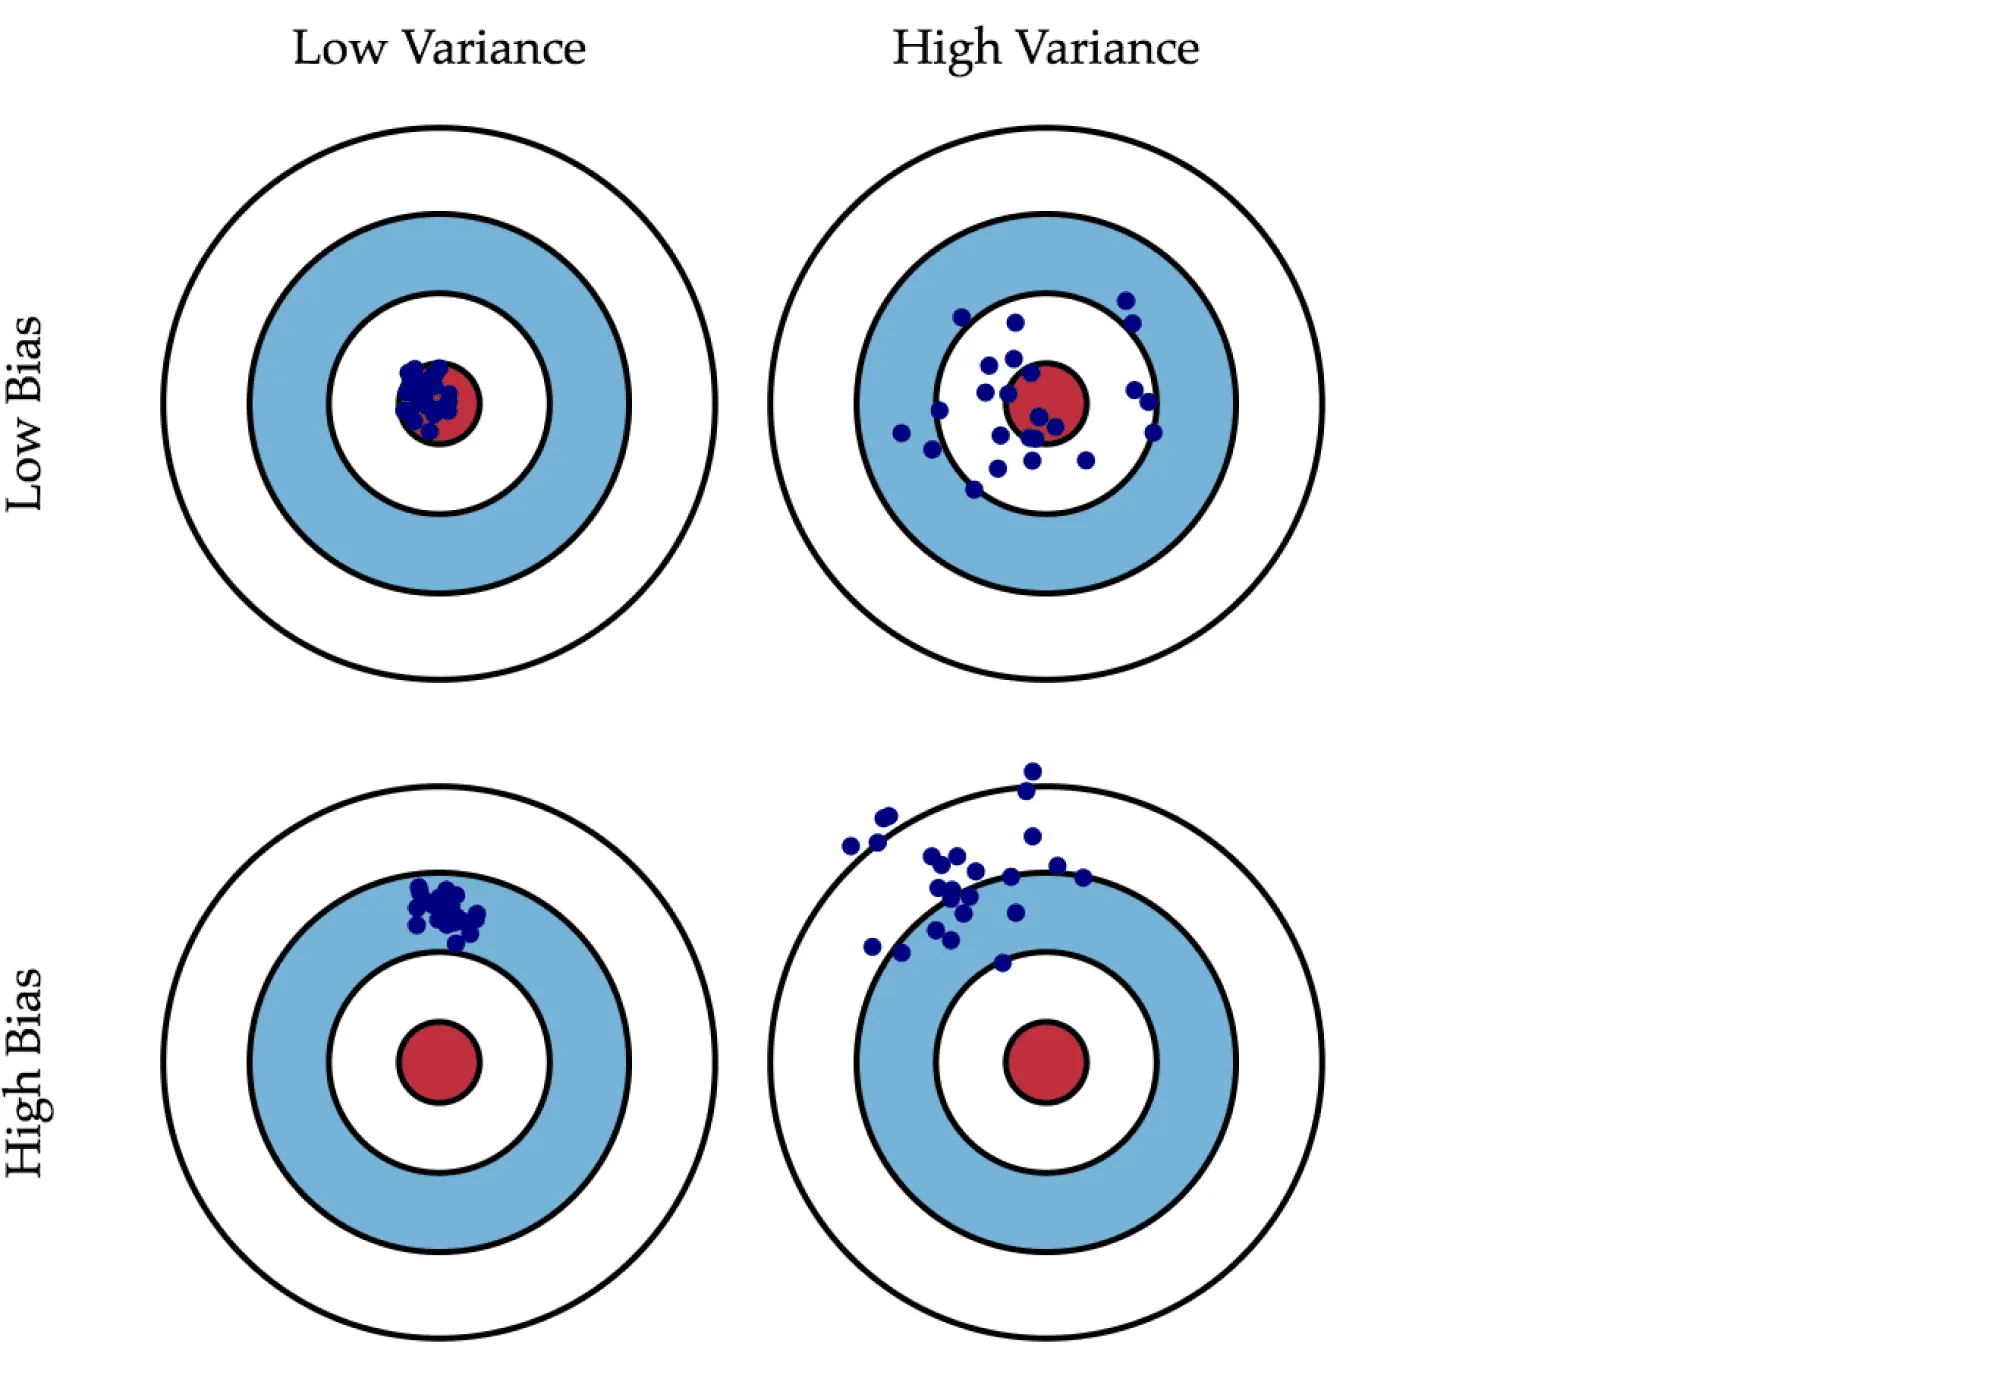
\includegraphics[width=1\linewidth]{img/bvd.png}
\end{figure}

При низком разбросе, но высоком смещении, мы видим, что выстрелы кучные, но все мимо "--- это и есть недообучение. Наша модель не слишком неадекватная, но при этом систематически <<попадает>> не туда.

При высоком разбросе, но низком смещении, мы вроде как <<попадаем>> туда, но наша <<стрельба>>, мягко скажем, не самая точная. Это объясняется переобучением: модель слишком сильно подстраивается под закономерности в данных, после чего не способна показать себя хорошо на новых данных.

В случае высокого смещения и высокого разброса, модель просто неадекватная. Модель выдаёт слишком разное, но при этом и близко не в той области, где должна. Обычно это свидетельствует о том, что модель поломана, то есть выдаёт абсолютно непредсказуемые и неинтерпретируемые значения.

\subsection*{Визуализация смещения и разброса}

Давайте рассмотрим деревья на разных наборах данных, и будем постепенно увеличивать их максимальную глубину (напомним, что за это отвечает параметр \texttt{max\_depth}:
\begin{figure}[H]
    \centering
    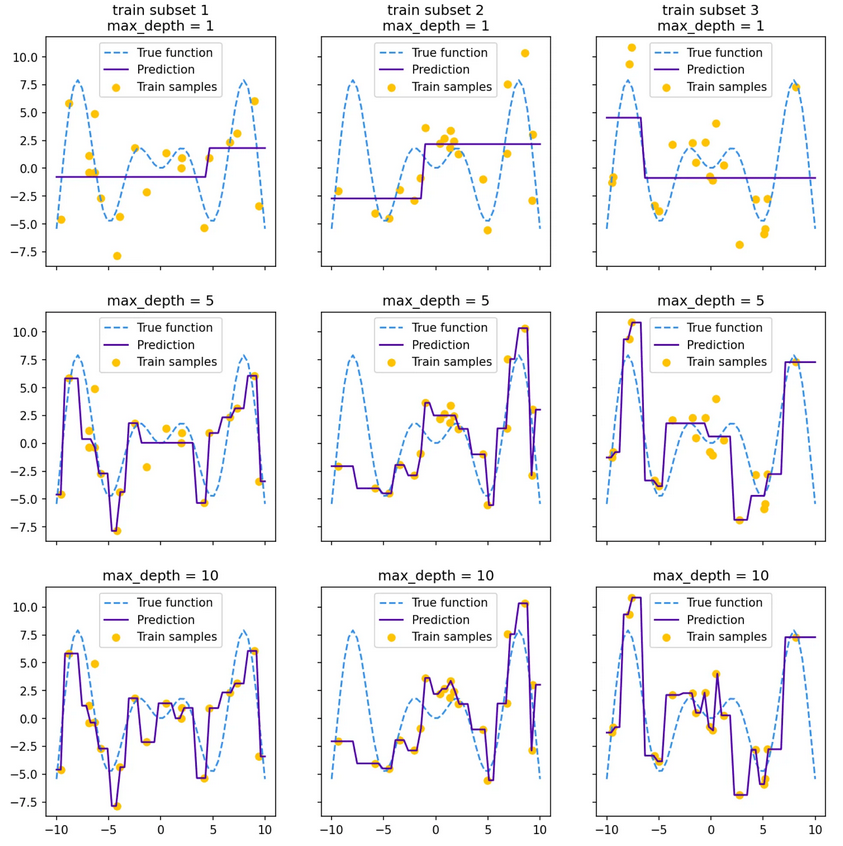
\includegraphics[width=1\linewidth]{img/bvd_tree.png}
\end{figure}

Как мы видим, при глубине $1$, наши деревья совсем ничего не улавливают в данных, а их прогнозы происходят где"=то мимо "--- это свидительствует о высоком смещении.

Давайте рассмотрим другой граничный случай, при глубине $10$. В таком случае, деревья слишком сильно адаптируются под данные. Проведём мысленный эксперимент: дорисуем ещё похожие точки и с лёгкостью убедимся, что модель многовероятно будет сильно ошибаться на них. Это и есть переобучение, которое является следствием из высокого разброса.

При глубине $5$ всё работает так, как мы и ожидаем "--- модель достаточно обучена, чтобы находить закономерности, и не слишком переобучена, чтобы не уметь предсказывать на новых данных. 